
\begin{comment}
\begin{frame}[plain]
\begin{center}
\textbf{\Large Recherche d'événements avec 4 quarks top}
\end{center}
\end{frame}
\end{comment}


\begin{frame}
\frametitle{Quark top et nouvelle physique}

\begin{columns}
\begin{column}{0.12\textwidth}
\hspace*{-1cm}
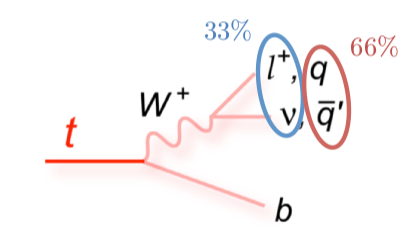
\includegraphics[width=2.2\textwidth]{Figures/FourTops/TopDecay.png}
\end{column}
\begin{column}{0.78\textwidth}
\begin{varblock}[8cm]{Quark top}
\begin{maliste}
\item[$\rightarrow$] Masse = $173,34\pm 0,76$~GeV
\item[$\rightarrow$] Fen\^etre sur EWSB
%\item Désintégration précède hadronisation
\item[$\rightarrow$] Désintégration ``facilement'' observable
\item[$\rightarrow$] Modes de production : paire, c\'elibataire
\end{maliste}
\end{varblock}
\end{column}
\hspace*{-1cm}
\begin{column}{0.1\textwidth}
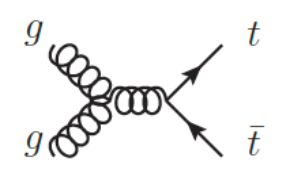
\includegraphics[width=1.6\textwidth]{Figures/FourTops/feyndiag_ttbar.png}\\
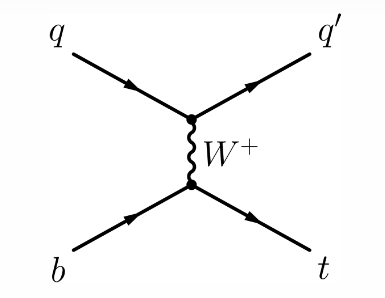
\includegraphics[width=1.5\textwidth]{Figures/FourTops/feyndiag_singletop_tchannel.png}
\end{column}
\end{columns}

\begin{center}
\hspace*{-1cm}
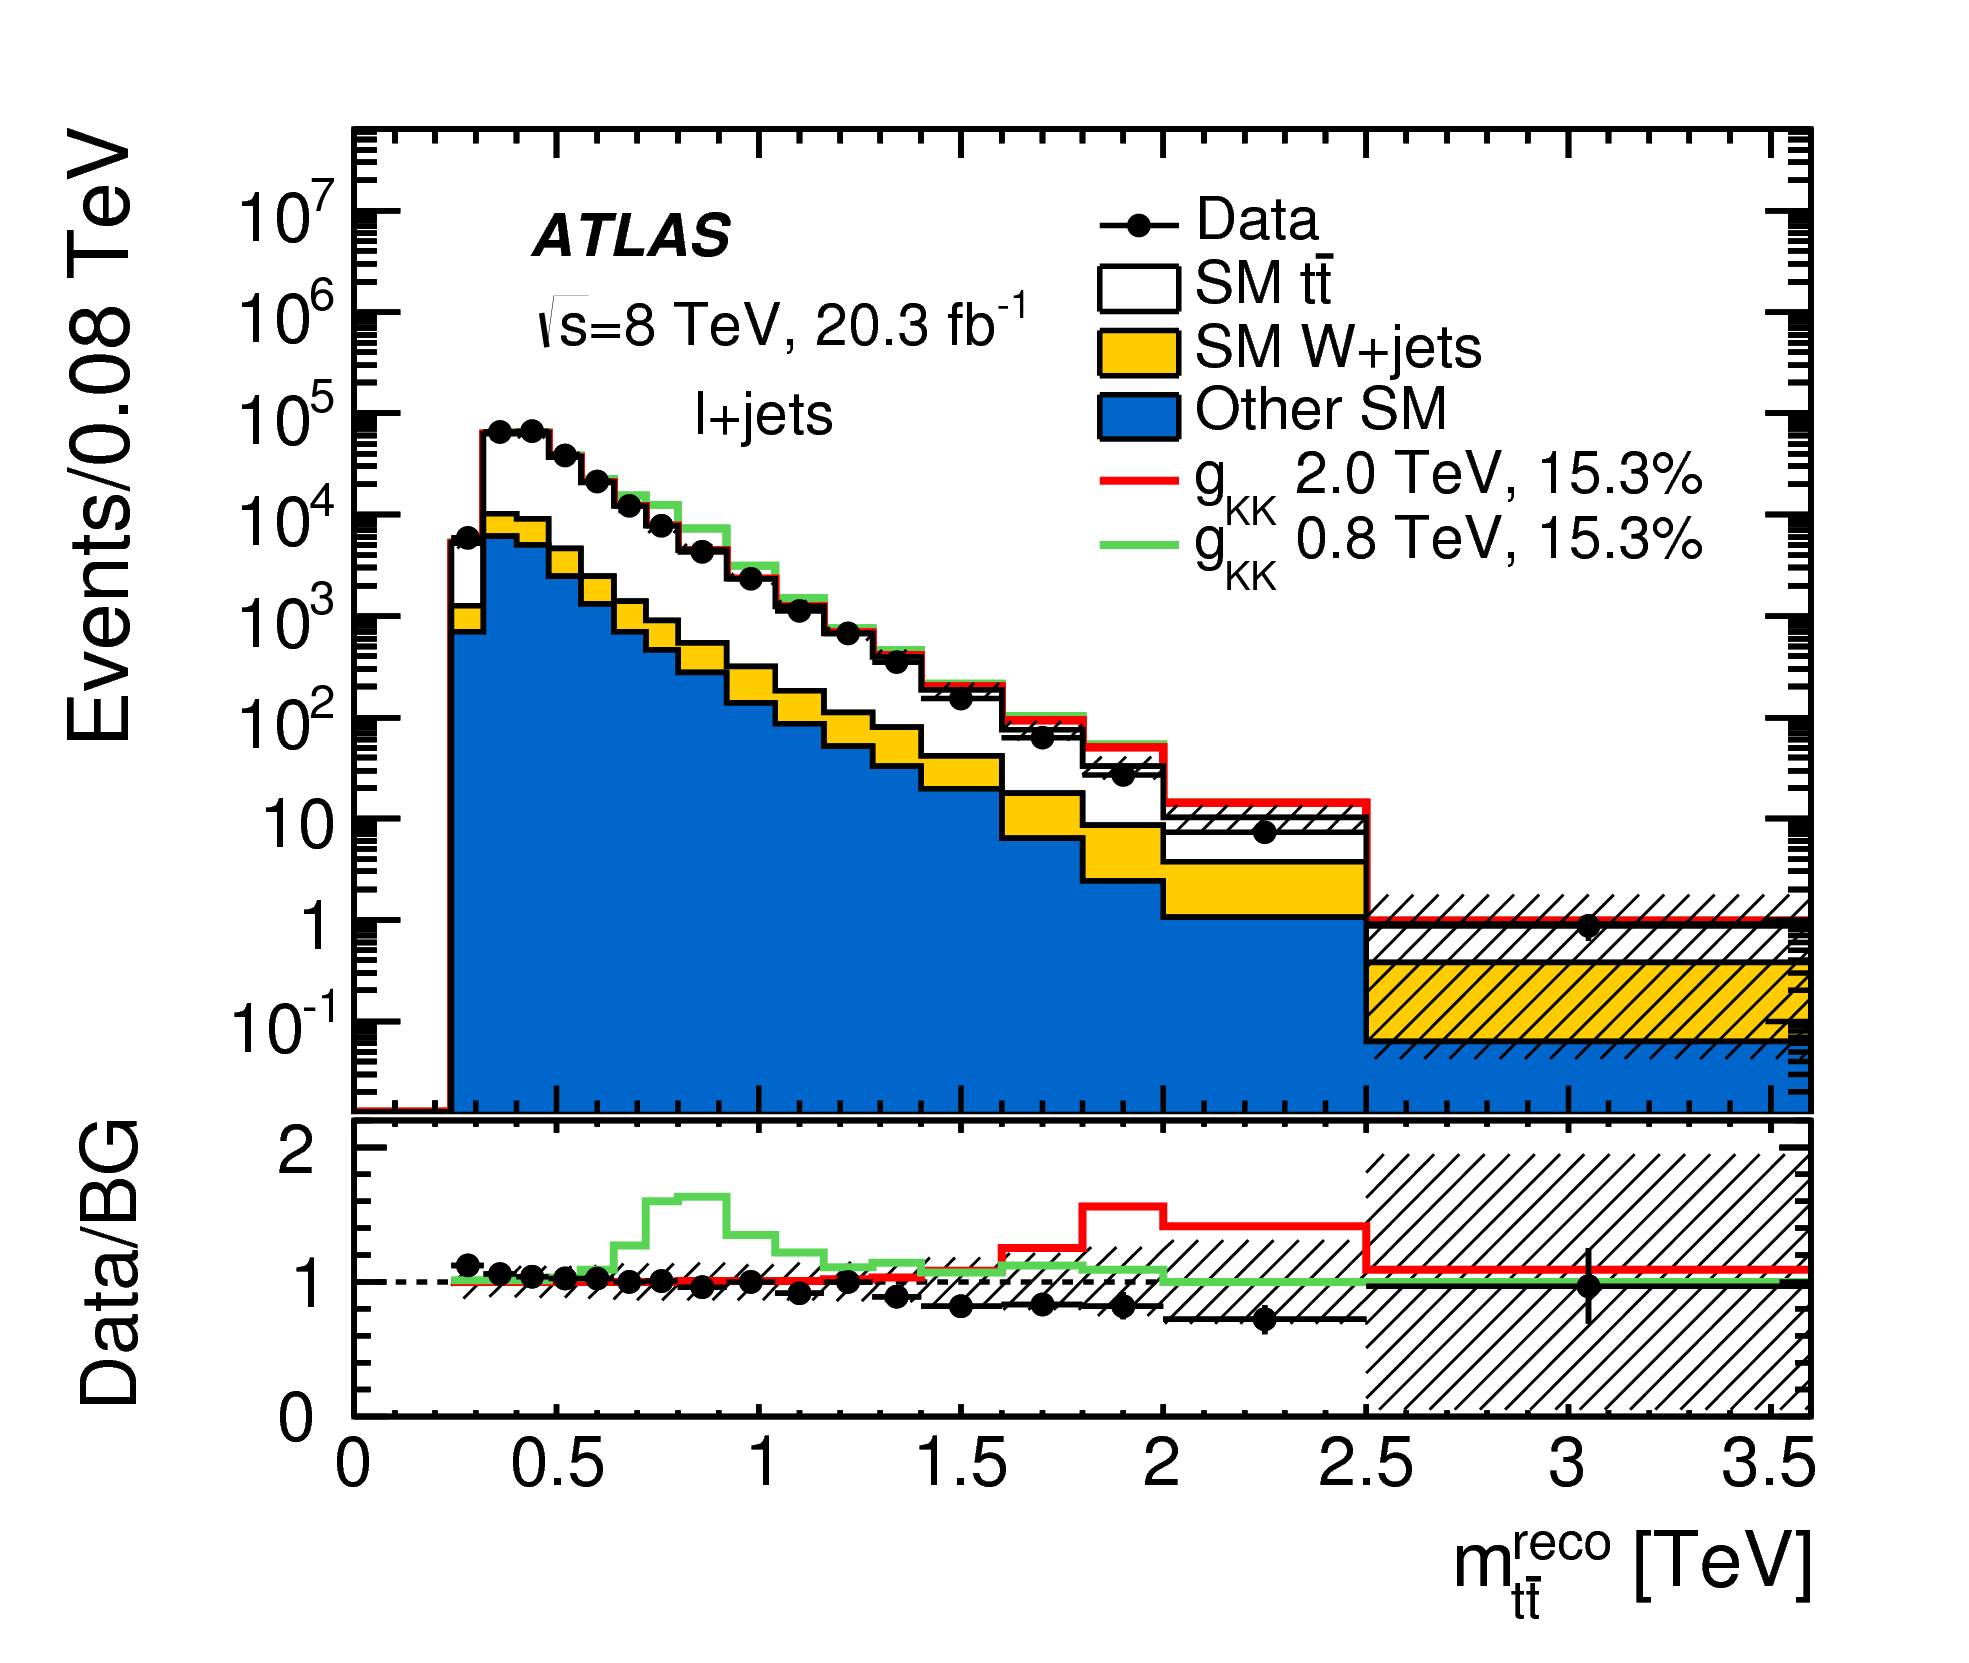
\includegraphics[width=0.3\textwidth]{Figures/FourTops/fig_resonancettbar.png}
\hspace*{-0.2cm}
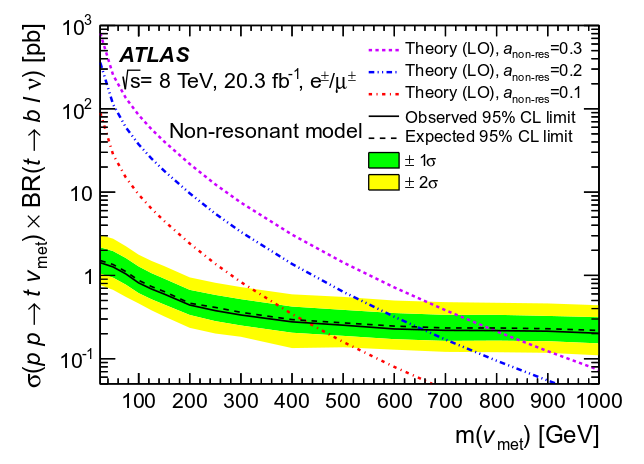
\includegraphics[width=0.35\textwidth]{Figures/FourTops/fig_monotop.png}%\\
%\vspace*{-0.5cm}
%\hspace*{1cm}
\hspace*{-0.15cm}
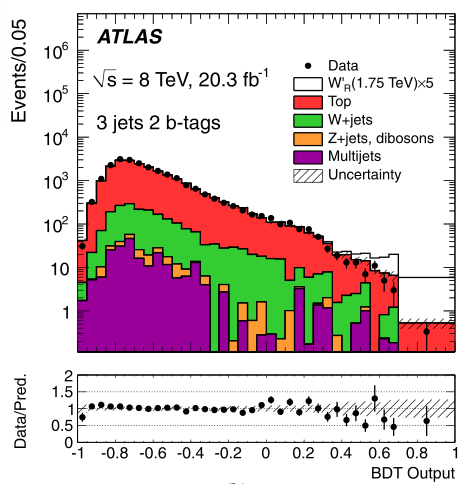
\includegraphics[width=0.23\textwidth]{Figures/FourTops/fig_Wprime.png}
\hspace*{-0.1cm}
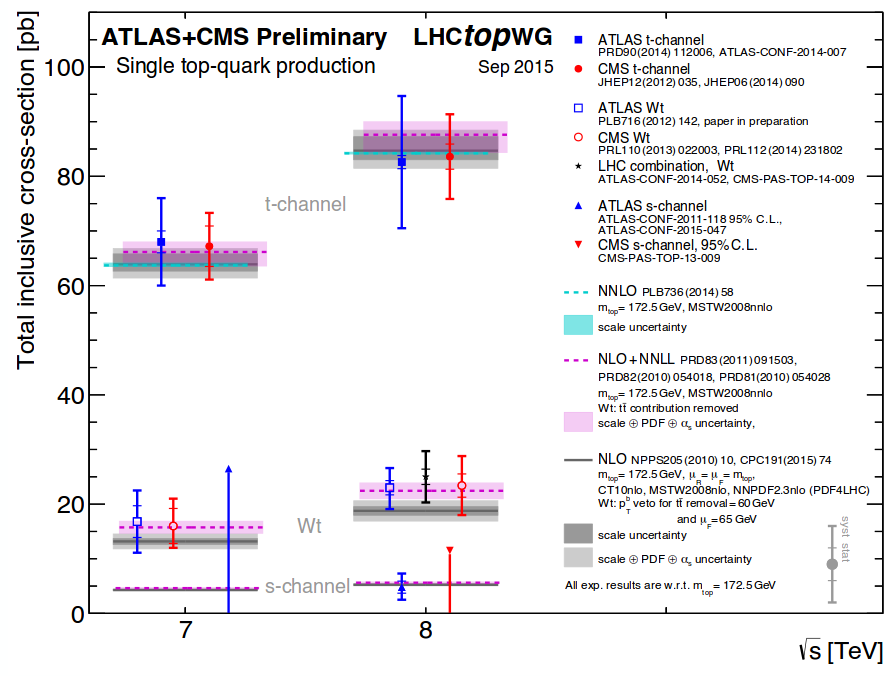
\includegraphics[width=0.3\textwidth]{Figures/FourTops/singletop_summaryplot.png}
\end{center}

\begin{maliste}
%\item Panorama des searches dans secteur du top (avec dimension historique) : top pair, single top (mettre plot ou valeurs xsec ?)
\item[$\rightarrow$] Nouveau mode de production : \'evénements 4 tops 
\begin{itemize}
\item Compl\'ementaire des autres modes de production
%Dire quelque chose sur complémentarité entre 4tops et les autres (single 
%top et top pair) : ex : 4tops par 2HDM peut apporter quelque chose par rapport 
%a ttbar car dans cas ttbar il y a interference importante qui peut rendre 
%analyse difficile
%\item Cet article peut etre interessant (pour voir mesures dans secteur du top qui sont utilisees pour contraindre les operateurs de nouvelle physique et le resultat de ces contraintes) : http://arxiv.org/pdf/1506.08845v1.pdf
\item LHC = premier labo permettant recherche 4 tops
%\item Pas si r\'ecents que cela ...
\end{itemize}
\end{maliste}
\end{frame}

\begin{frame}
\frametitle{}
\begin{center}
\vspace*{-0.7cm}

\includegraphics[width=1\textwidth]{Figures/FourTops/TheFourTopsMusic.jpg}
\end{center}
\end{frame}

\begin{comment}
\begin{frame}
\frametitle{Historique}

\begin{figure}[!htb]
\begin{center}
\vspace*{-0.8cm}
%\vspace*{-1cm}
\hspace*{-0.5cm}
\includegraphics<1>[width=1.13\textwidth]{friseChrono4tops_1.pdf}
\vspace*{-5cm}
\hspace*{1cm}
\includegraphics<1>[width=0.4\textwidth]{Figures/FourTops/4topCalculationsFromBarger91.png}
\includegraphics<2>[width=1.13\textwidth]{friseChrono4tops_2.pdf}
\includegraphics<3>[width=1.13\textwidth]{friseChrono4tops_3.pdf}
\end{center}
\end{figure}
\end{frame}
\end{comment}

\begin{frame}
\frametitle{Historique}

\begin{figure}[!htb]
\begin{center}
\vspace*{-0.8cm}
%\vspace*{-1cm}
\hspace*{-0.5cm}
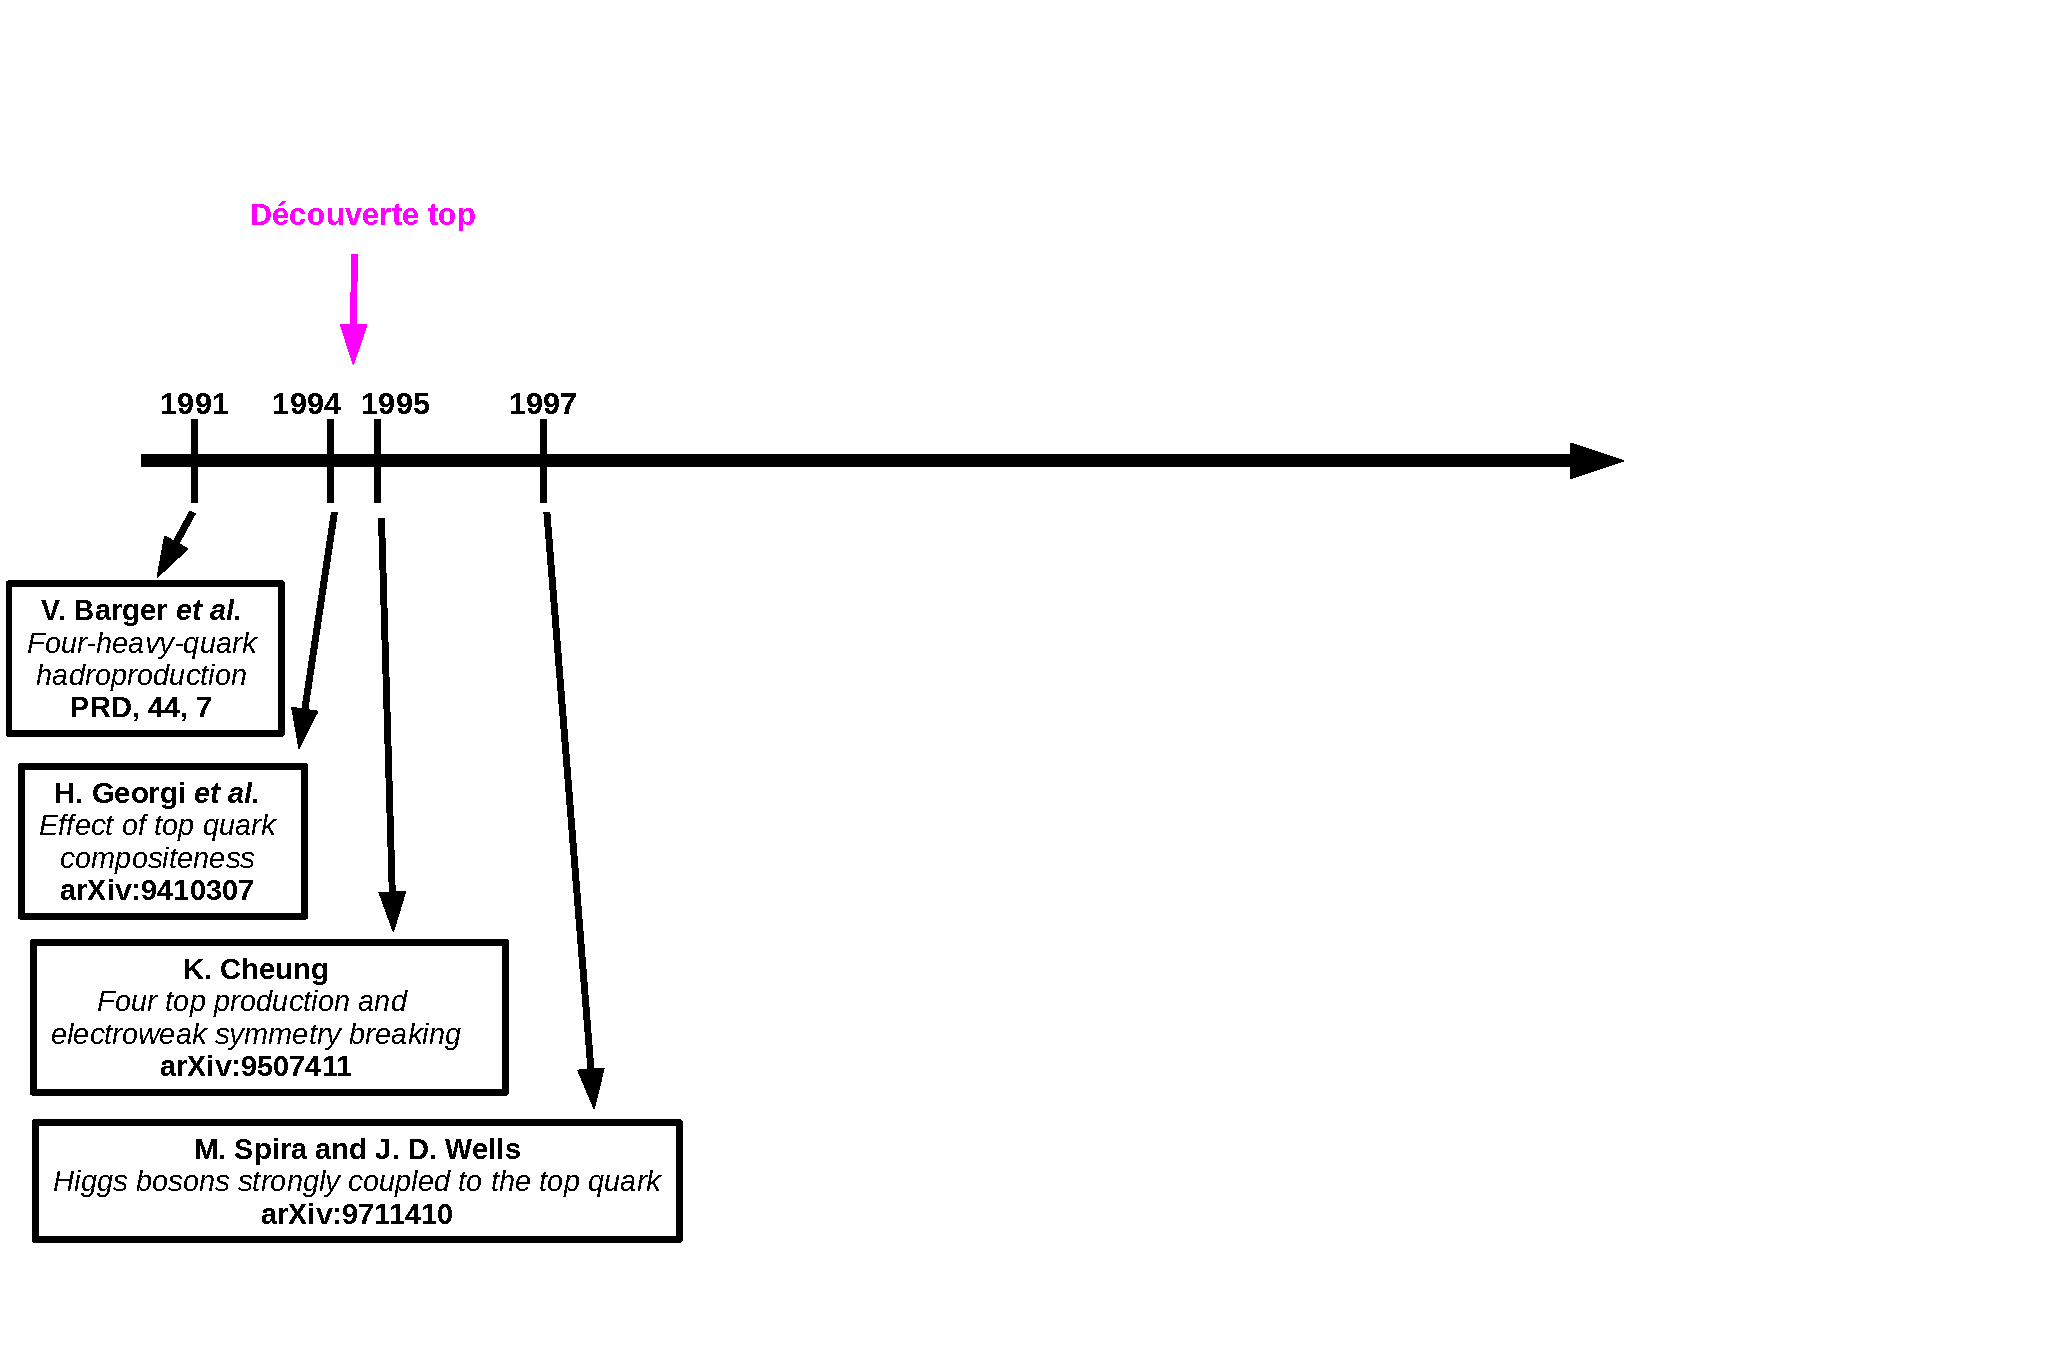
\includegraphics[width=1.13\textwidth]{friseChrono4tops_1.pdf}
\vspace*{-5cm}
\hspace*{1cm}
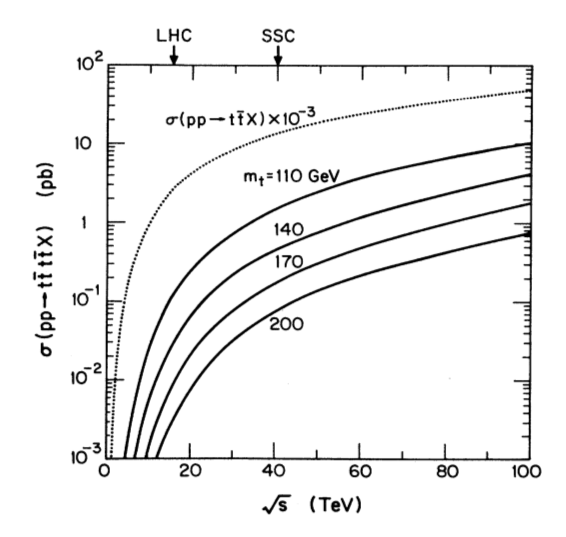
\includegraphics[width=0.4\textwidth]{Figures/FourTops/4topCalculationsFromBarger91.png}
\end{center}
\end{figure}
\end{frame}

\begin{frame}
\frametitle{Historique}
\begin{figure}[!htb]
\begin{center}
\vspace*{-0.5cm}
%\vspace*{-1cm}
\hspace*{-0.5cm}
\includegraphics<1>[width=1.13\textwidth]{friseChrono4tops_2test.pdf}
\includegraphics<2>[width=1.13\textwidth]{friseChrono4tops_3testarticleref.pdf}
\end{center}
\end{figure}
\end{frame}
